\chapter{CD Modelling}
\section{Introduction and Technical Background}
Battery enclosures are critical components in the design of energy storage systems, particularly in mobile and compact applications. They serve as structural containers for lithium-ion cells and provide necessary protection against environmental and mechanical influences. Their design must reconcile several competing requirements: mechanical robustness, thermal management, electrical insulation, compactness, and manufacturability. With the increasing adoption of 3D printing technologies, engineers now have more flexibility to prototype and produce such enclosures, particularly for small-series or custom applications \cite{gebhardt2016}.

Modern lithium-ion cells come in standardized formats, such as cylindrical (e.g., 18650), prismatic, or pouch cells. Each of these formats imposes specific geometric and thermal constraints on the enclosure. Cylindrical cells, for example, are highly space-efficient in tightly packed arrays but require firm fixation and vibration dampening, as well as thermal spacing to avoid overheating. Enclosures for such cells often include integrated cell holders, structural ribs, and defined cooling pathways \cite{pistoia2018}. 

An essential consideration in battery pack design is thermal management. Since lithium-ion batteries are sensitive to excessive heat, the enclosure must ensure proper heat dissipation. Passive solutions, such as airflow channels or thermally conductive plastics, can be incorporated into the design. In high-performance applications, the enclosure may include embedded cooling elements. The thermal behavior of the entire assembly must be taken into account early in the design phase to avoid heat accumulation and ensure battery safety and longevity.

Mechanical constraints also play a decisive role. Battery packs are often subjected to vibration, shocks, and compression forces. Therefore, the housing material must be both strong and lightweight. Common materials used in 3D printing for such applications include ABS, PETG, and polyamide (PA12), each of which offers a specific balance of mechanical resilience, thermal resistance, and printability \cite{gebhardt2016}.

The enclosure design must also accommodate connectors, cable guides, ventilation openings, and possibly fasteners for mounting within a device or vehicle. All of these features must be precisely aligned and dimensioned to ensure a secure and reliable assembly. Such complexity makes parametric and constraint-based design software particularly valuable.

\section{Design Approach Using Fusion 360}
Autodesk Fusion 360 provides an integrated environment for computer aided design (CAD), simulation, and Computer-Aided Manufacturing (CAM), which makes it particularly well-suited for iterative design and prototyping of technical components like battery enclosures. Its parametric modeling capabilities allow engineers to define the relationships between different parts of the geometry, ensuring that dimensional adjustments propagate automatically throughout the model \cite{hogan2025}.

Using Fusion 360, a designer can first define a master sketch that includes key dimensions such as cell spacing, wall thickness, and screw positions. Through extrusion and patterning, these base geometries are transformed into 3D solids. Additional features such as ventilation slots or mounting flanges can be added using derived sketches and Boolean operations\cite{hogan2025}..

Assemblies in Fusion 360 enable designers to position and constrain battery cells within the enclosure, simulating real-world configurations. This allows for spatial validation and interference checking early in the process, reducing the risk of design flaws during manufacturing\cite{hogan2025}..

Moreover, Fusion 360 supports exporting the final design directly into formats suitable for additive manufacturing, such as STL or 3MF. This integration streamlines the workflow from design to production, making it ideal for rapid prototyping and validation\cite{hogan2025}..

From a manufacturability perspective, the designer must also follow principles of Design for Additive Manufacturing (DfAM). This includes minimizing unsupported overhangs, ensuring even wall thicknesses, and aligning features for optimal layer orientation. Fusion 360 offers visualization tools and slicer integration to help evaluate the printability of the part \cite{anderson2020}.

In summary, Fusion 360 offers the necessary flexibility and functionality to develop complex battery enclosures that meet structural, thermal, and electrical requirements. Its parametric design environment, combined with visualization and export tools, makes it an effective platform for realizing functional prototypes that are ready for testing and refinement.

\section{Design and Development of a Modular Lithium-Ion Battery System}

The design illustrates a modular lithium-ion battery storage system, developed for high-density energy applications such as stationary energy storage, backup infrastructure, or mobile electrification platforms. The system is based on 21700-format lithium-ion cells, arranged in a densely packed structural configuration to optimize both volumetric energy density and thermal dissipation properties. The design process was carried out using CAD modeling tools, including parametric 3D assemblies, with iterative thermal and structural simulations executed to ensure mechanical and thermal stability under nominal and elevated load conditions.

\section{Introduction}

The design of battery housings is an essential step in developing reliable energy storage systems. Autodesk Fusion 360 offers an integrated CAD environment ideal for creating precise and adaptable models, especially when targeting additive manufacturing methods. This section focuses on the detailed process of creating, structuring, and refining battery enclosure CAD files within Fusion 360, emphasizing parametric design and manufacturability \cite{hogan2025}.

\section{Parametric Modeling Principles}

Parametric modeling underpins efficient design workflows in Fusion 360. By defining key dimensions and constraints as parameters, changes can be propagated throughout the model automatically. This approach enables rapid iteration and consistent accuracy across complex geometries \cite{anderson2020}.

Initial modeling begins with sketches representing cross-sectional profiles of the battery cells and enclosure features. These sketches are converted into 3D geometry via extrusion, revolution, or other solid modeling operations. Parameters controlling dimensions such as cell diameter, wall thickness, and sensor pocket size are set at the outset, allowing easy adjustments during development \cite{gebhardt2016}.

\section{Base Geometry and Cell Arrangement}

The first step is designing the footprint to hold the battery cells securely. For cylindrical 18650 cells, a circular sketch with a diameter of 18.6 mm is created. To accommodate tolerances and thermal expansion, an additional clearance of approximately 1.5 to 2 mm is added around each cell \cite{pistoia2018}. Using Fusion 360’s pattern features, this base slot is duplicated to form the desired cell matrix arrangement.

Next, the outline of the overall enclosure is sketched, defining the external boundaries. The sketch is extruded to form the base structure, with wall thickness set according to mechanical strength requirements and printability constraints, typically ranging from 2 mm to 4 mm \cite{gebhardt2016}.

\section{Feature Addition: Sensor Integration and Cable Management}

A critical aspect of the enclosure design is the integration of temperature sensors. Dedicated pockets are created by cutting recesses adjacent to the battery cells using parametric cut operations. These pockets are dimensioned to fit common thermistors or digital sensors securely, ensuring reliable thermal contact \cite{anderson2020}.

Additionally, routing channels for sensor wiring are incorporated into the design. These channels prevent wire interference and facilitate clean assembly. All such features are parameter-driven, allowing dimension adjustments as sensor specifications or wiring requirements evolve.

\section{Assembly Modeling and Component Placement}

Fusion 360’s assembly workspace enables importing battery cell and sensor component models. These are positioned within the enclosure to verify fit, clearances, and spatial relationships. The assembly environment supports the use of constraints and joints, allowing realistic simulation of component interactions \cite{hogan2025}.

Parameters controlling cell spacing, sensor pocket depth, and cable routing pathways are globally defined. Altering any parameter updates the entire assembly model, significantly improving design iteration speed and accuracy.

\section{Design for Additive Manufacturing (DfAM) Considerations}

Throughout the modeling process, adherence to DfAM principles is crucial to ensure manufacturability via 3D printing. This includes minimizing overhangs exceeding recommended angles (usually 45°), maintaining uniform wall thickness to prevent warping, and designing features to reduce the need for support material \cite{anderson2020}.

Fillets and chamfers are strategically applied to edges to improve mechanical strength and printing quality. The model is split into modular subassemblies where necessary, facilitating multi-part printing and post-processing.

\section{Manufacturing Preparation and Export}

The final step in the design workflow involves exporting the CAD files into formats compatible with slicing software, primarily STL or 3MF \cite{gebhardt2016}. Fusion 360’s built-in manufacturing tools allow users to simulate print jobs, preview layer-by-layer builds, and optimize part orientation for strength and surface finish.

Subsequent iterations incorporate feedback from prototype prints, with dimension adjustments made via the parametric model to fine-tune fit and function.

\section{Iterative Refinement and Version Control}

Due to the parametric nature of the model, any necessary refinements—such as modifying sensor pocket sizes or wall thickness—are efficiently implemented without reconstructing the design from scratch \cite{hogan2025}. Fusion 360’s version control system aids in tracking changes and managing design variants.

This iterative design methodology accelerates development timelines and reduces errors, particularly when integrating complex features like sensor integration and wiring management.



\section{Application Context: Battery Housing for the E-Mule Energy Storage System}
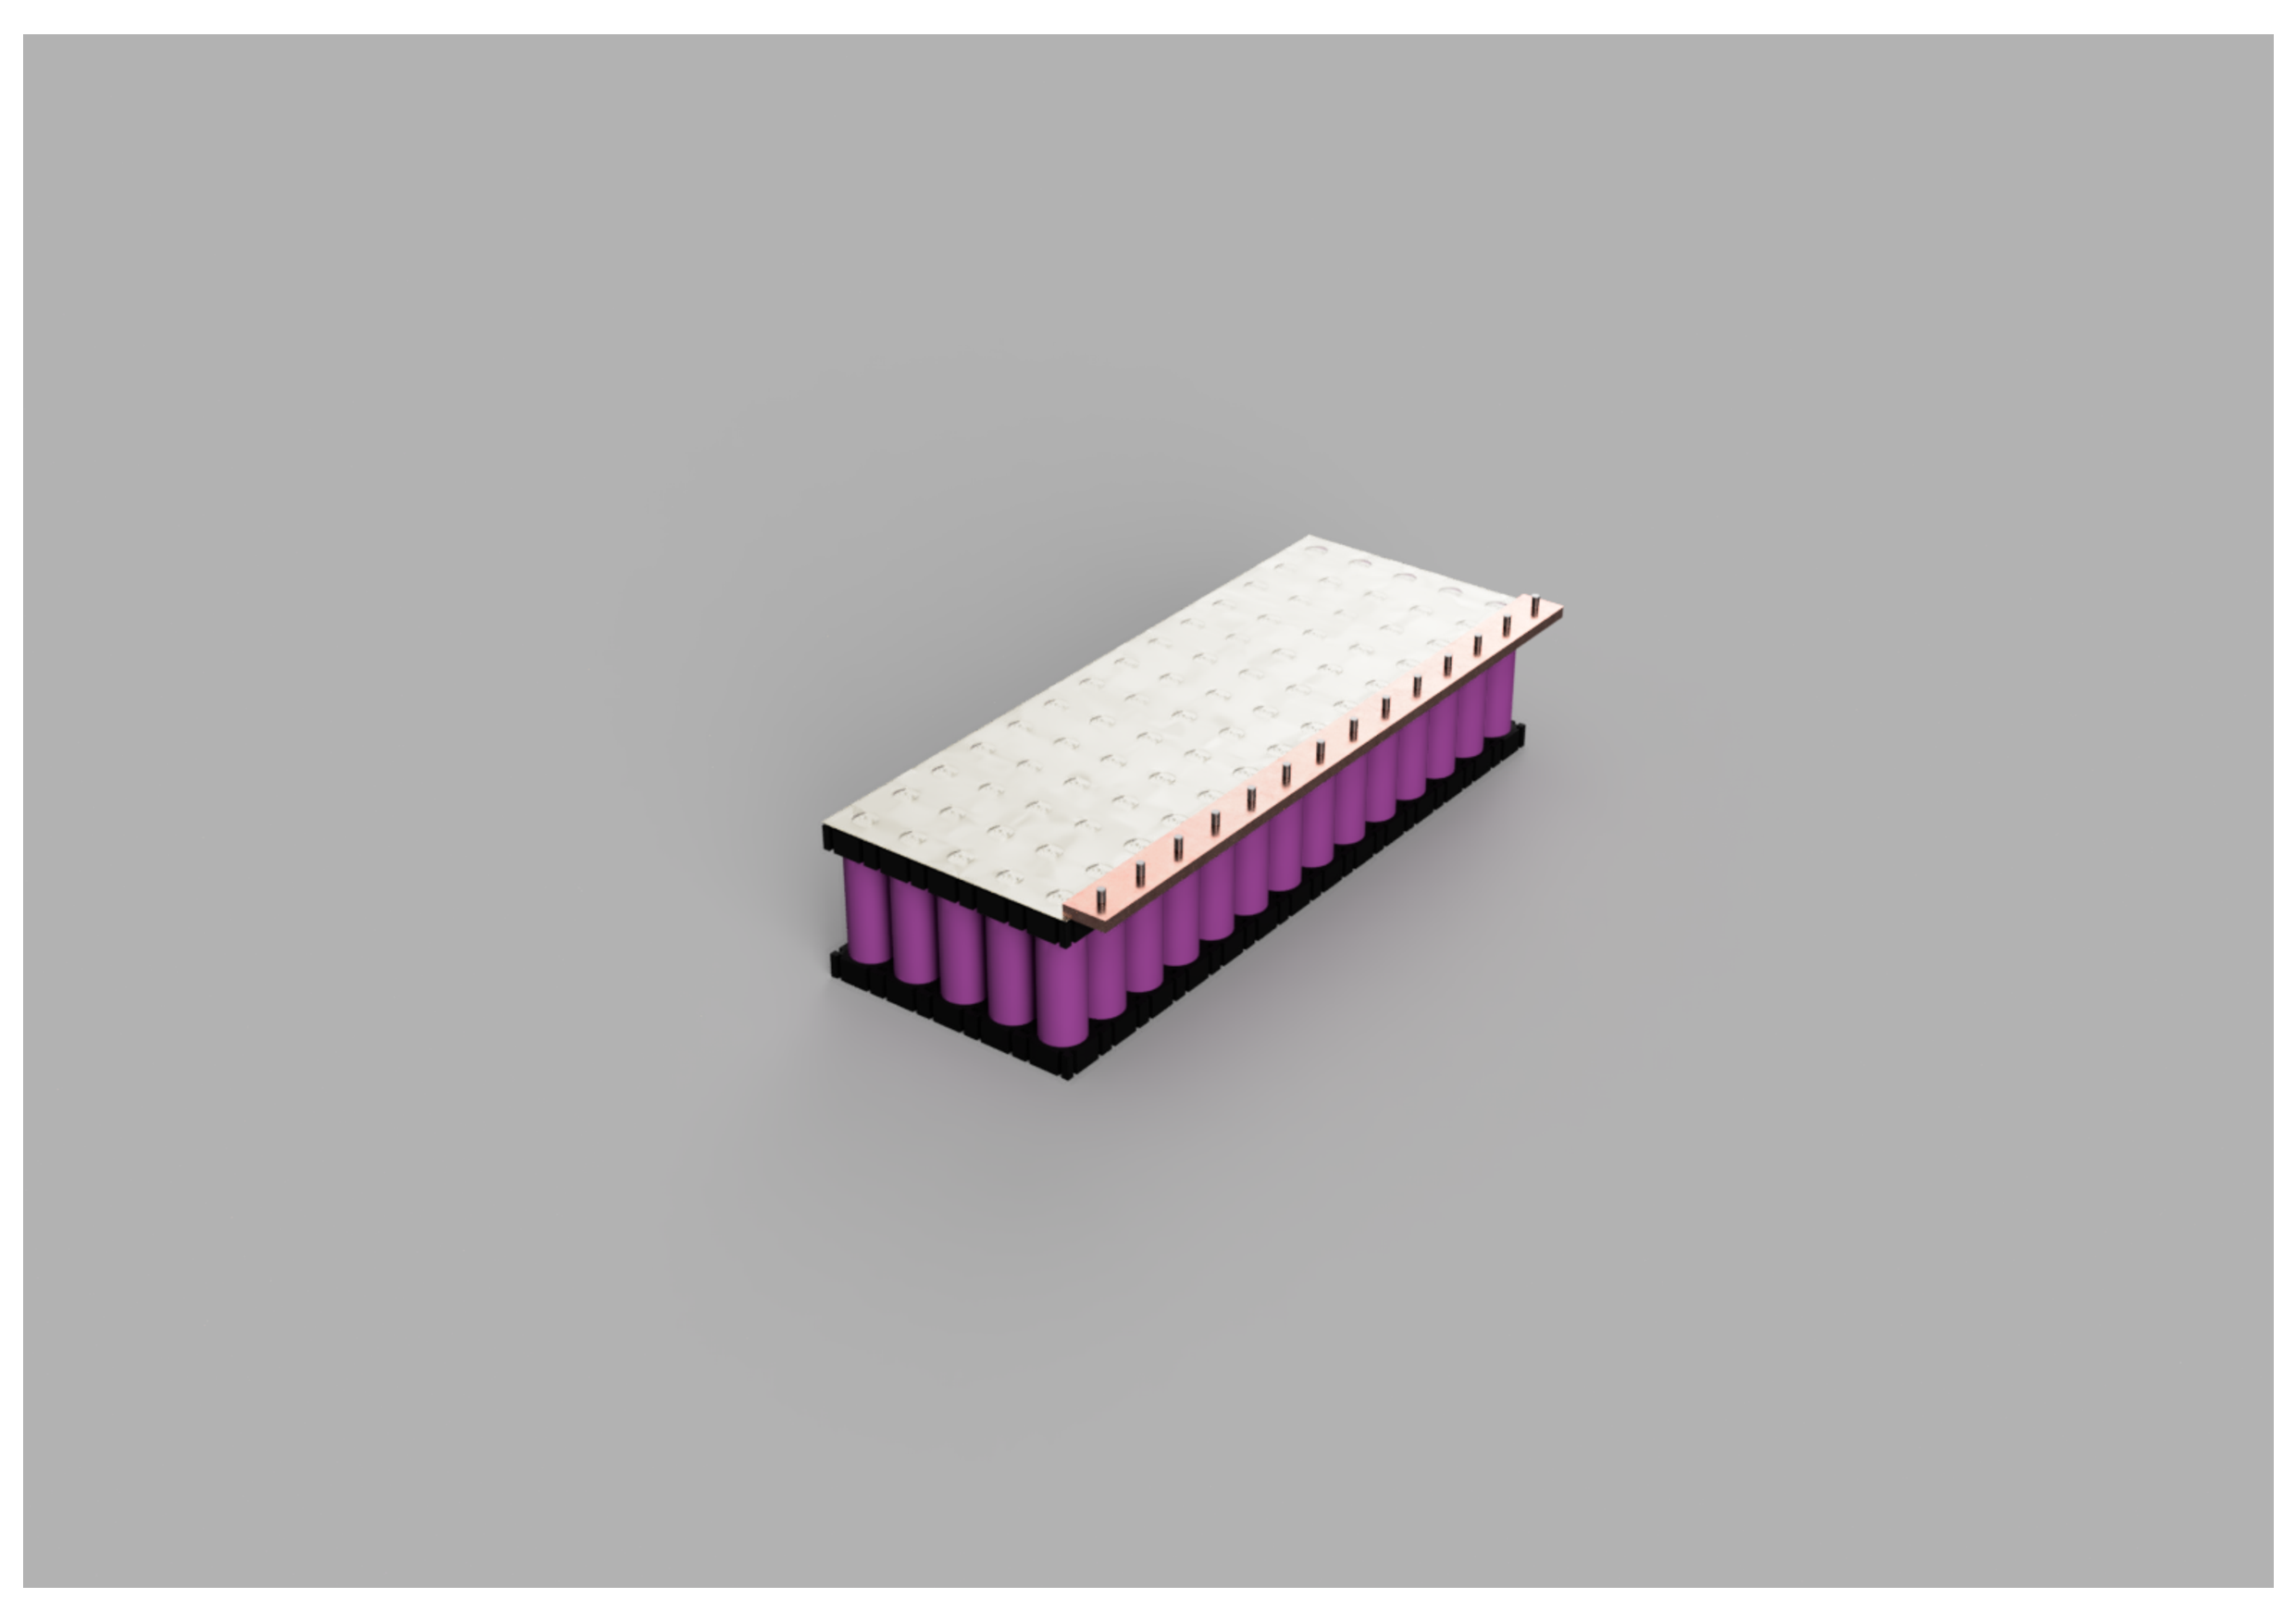
\includepdf[pages=1, fitpaper=true, pagecommand={%
	\thispagestyle{empty} % Entfernt Seitenzahlen und Kopfzeilen
	\begin{center}
		\captionof{figure}{etailed 3D CAD rendering of a lithium-ion cell used in the energy storage system.} % Fügt die Caption ein
		\label{fig:Zelle} % Für Querverweise
	\end{center}
}]{circuts/Zelle.pdf}
\addtocounter{page}{1} % Seitenzähler korrekt erhöhen

The battery pack presented in \ref{fig:Zelle}  was designed specifically for use in an electric utility vehicle—the E-Mule. In such mobile applications, energy storage must not only provide sufficient capacity and power density, but also fulfill mechanical and thermal requirements, ensure serviceability, and allow compact packaging. These constraints played a central role in the CAD modeling process and directly influenced key design decisions.

The final design was entirely created using Fusion 360, with a strong focus on modularity, manufacturability, and the physical integration of standard lithium-ion cells (type 21700). The enclosure and internal structures were tailored for additive manufacturing using PETG, a common thermoplastic with suitable strength and heat resistance \cite{gebhardt2016}. No electrical testing or thermal simulation was conducted as part of this stage; the focus remained on the mechanical layout and enclosure architecture.

\section{Detailed CAD Design Process in Fusion 360}

\subsection{Cell Holder Design and Arrangement}

The first modeling step was the design of an individual battery cell holder (\ref{fig:Zelle}). Each cell is a cylindrical 21700 lithium-ion battery, typically 21 mm in diameter and 70 mm in length. In Fusion 360, a 2D sketch was created with circular cutouts for each cell, spaced evenly in a grid pattern. These cutouts were then extruded to form vertical cavities, which securely hold the cells while leaving sufficient clearance for thermal expansion and wiring.

To ensure consistent wall thickness and clearance, the design used parameterized dimensions tied to a master sketch. This allowed rapid iteration and adjustment of the number of cells in the matrix. 

The resulting layout provides space for a total of 70 cells (14× 5 array), which was deemed sufficient for the E-Mule’s use case in terms of energy content. The precision and symmetry of the layout were maintained through pattern tools and the use of midplane construction lines.

% Assembly mit Gehäuse
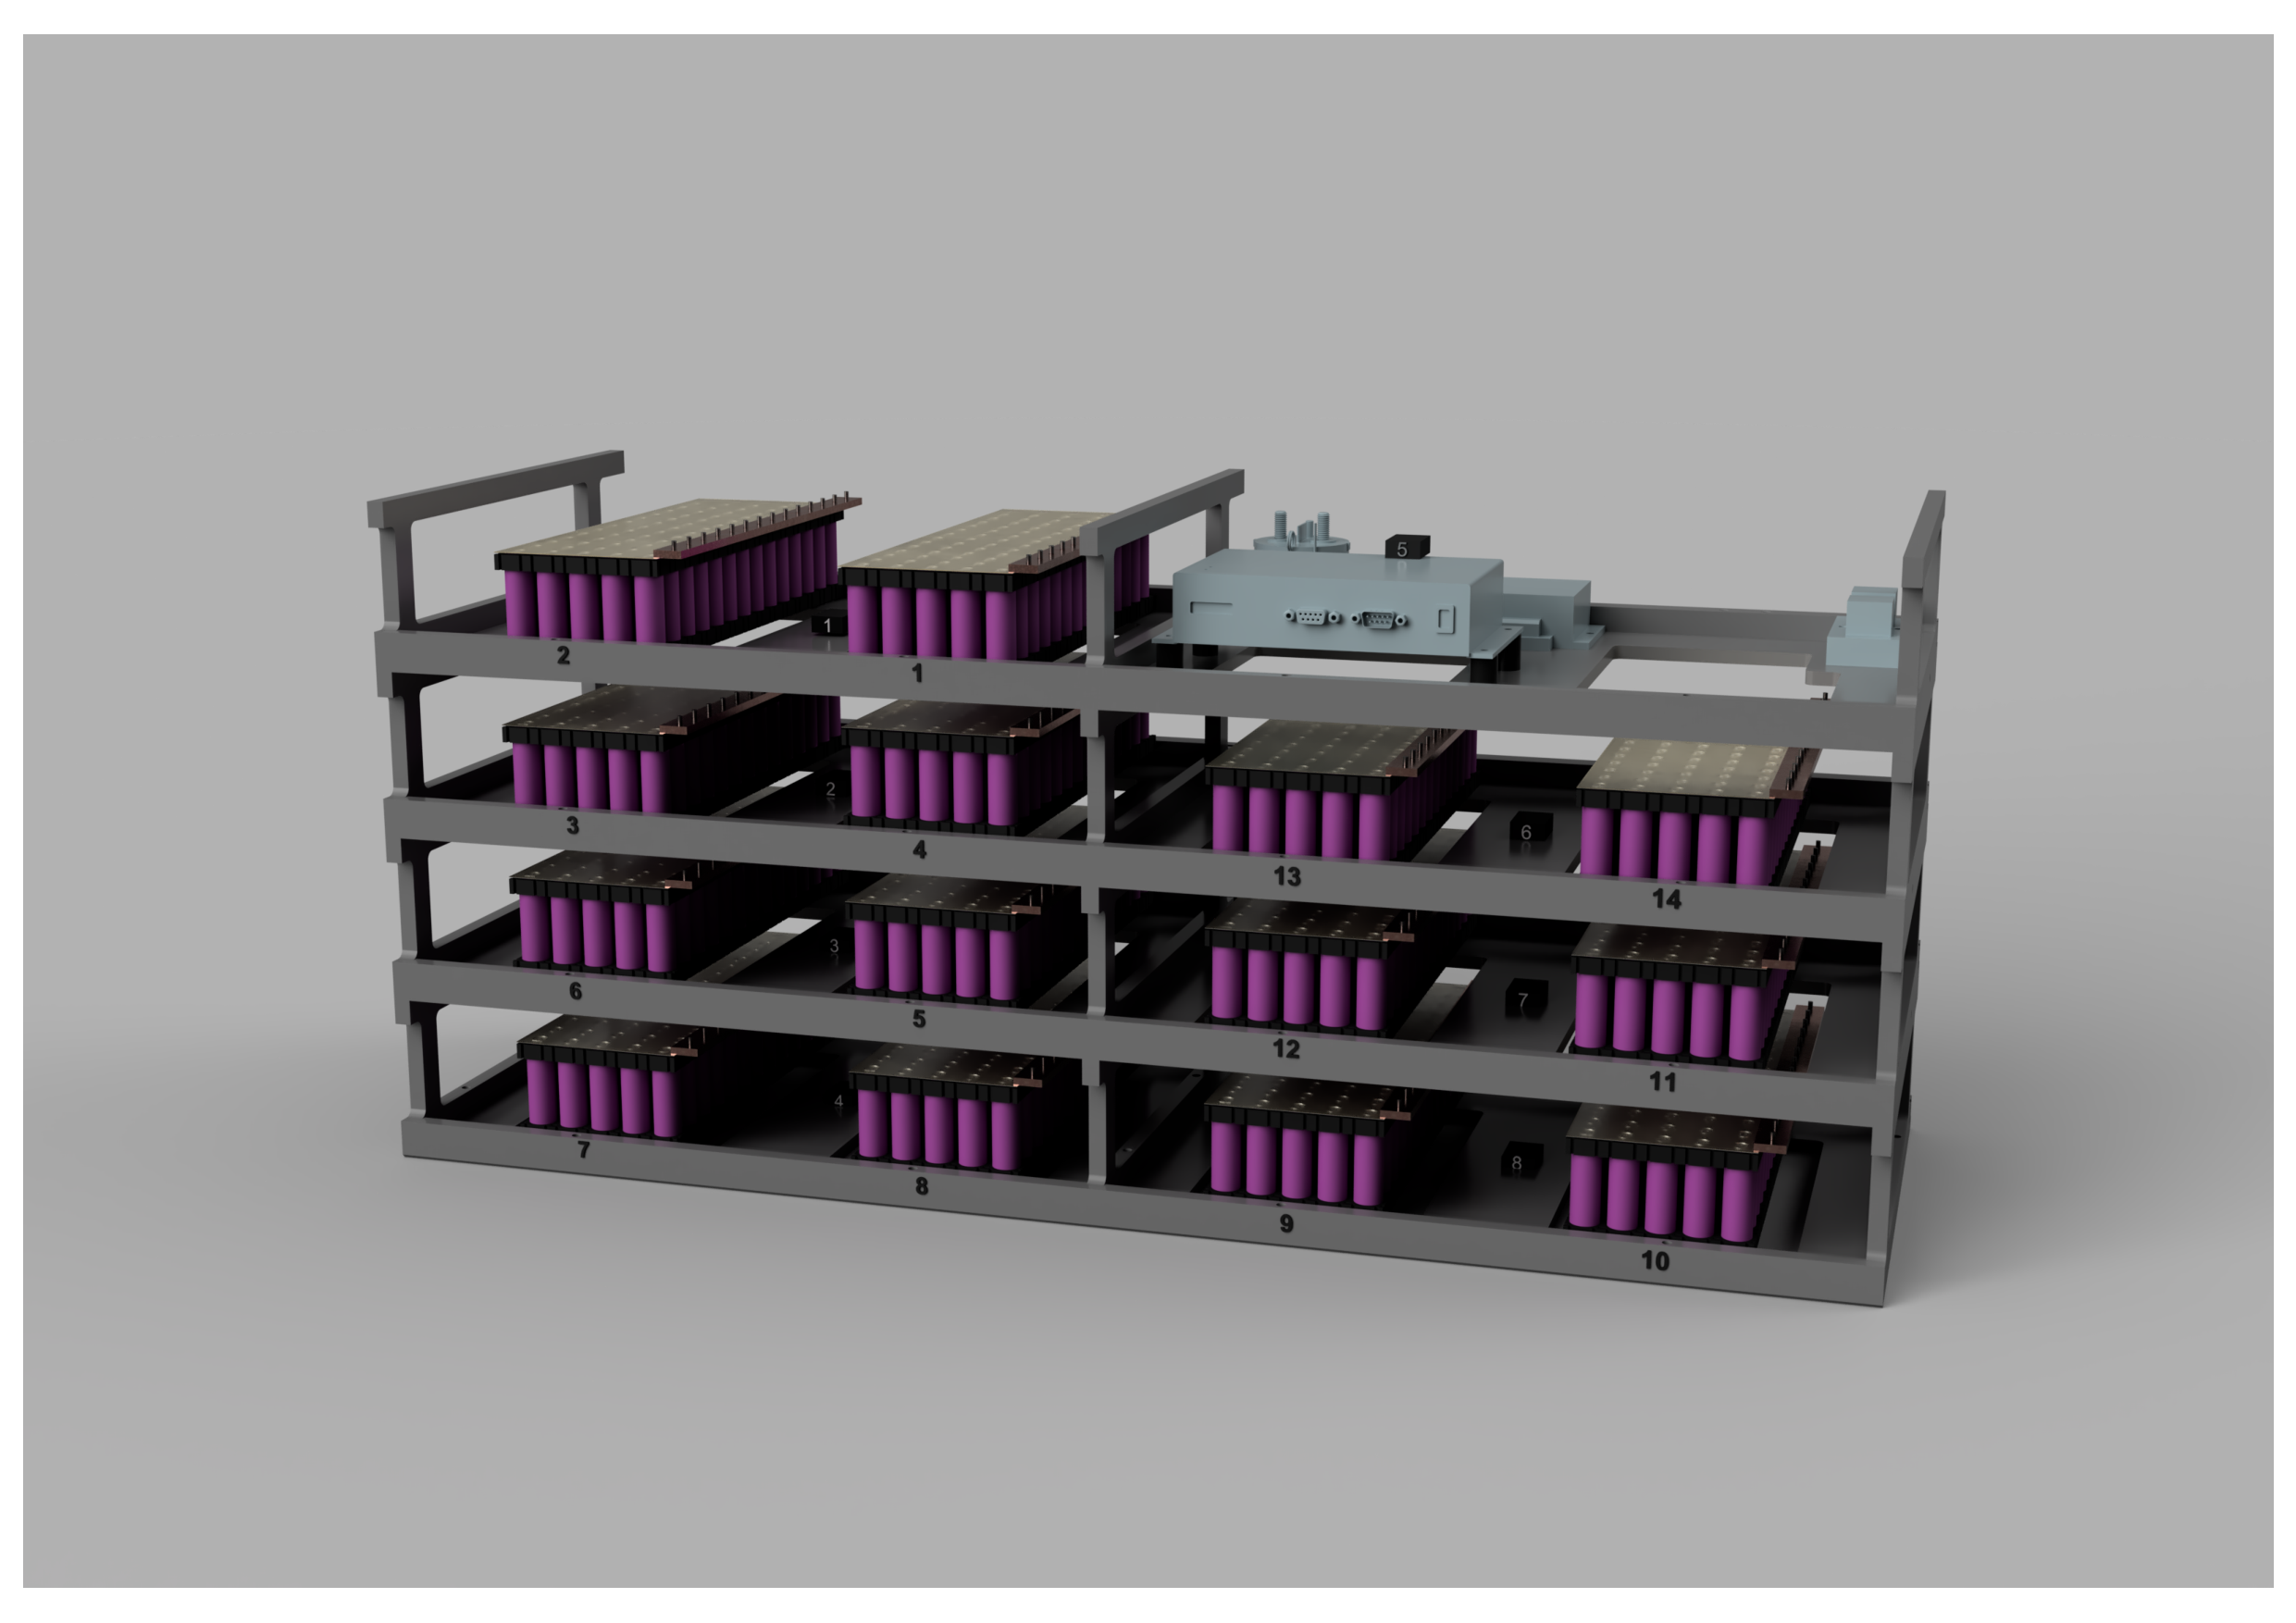
\includepdf[pages=1, fitpaper=true, pagecommand={%
	\thispagestyle{empty}
	\begin{center}
		\captionof{figure}{Fully assembled energy storage module.}
		\label{fig:Assembly}
	\end{center}
}]{circuts/Energiespeichersystem_Assembley_TOP.pdf}
\addtocounter{page}{1}

After creating the single cell holder as a component, it was duplicated and arranged in Fusion 360’s assembly environment to simulate the full module layout, seen in \ref{fig:Assembly}. This stage focused on integrating all components—holders, cell blocks, connector slots, sensor openings—into a complete mechanical structure.


During assembly, care was taken to maintain access to each row for both cooling and cabling. Clearances were checked using section analysis and interference detection tools within Fusion 360. Dummy models of power connectors and temperature sensors were placed to simulate real-world installation.



\subsection{Integration of the Protective Enclosure}
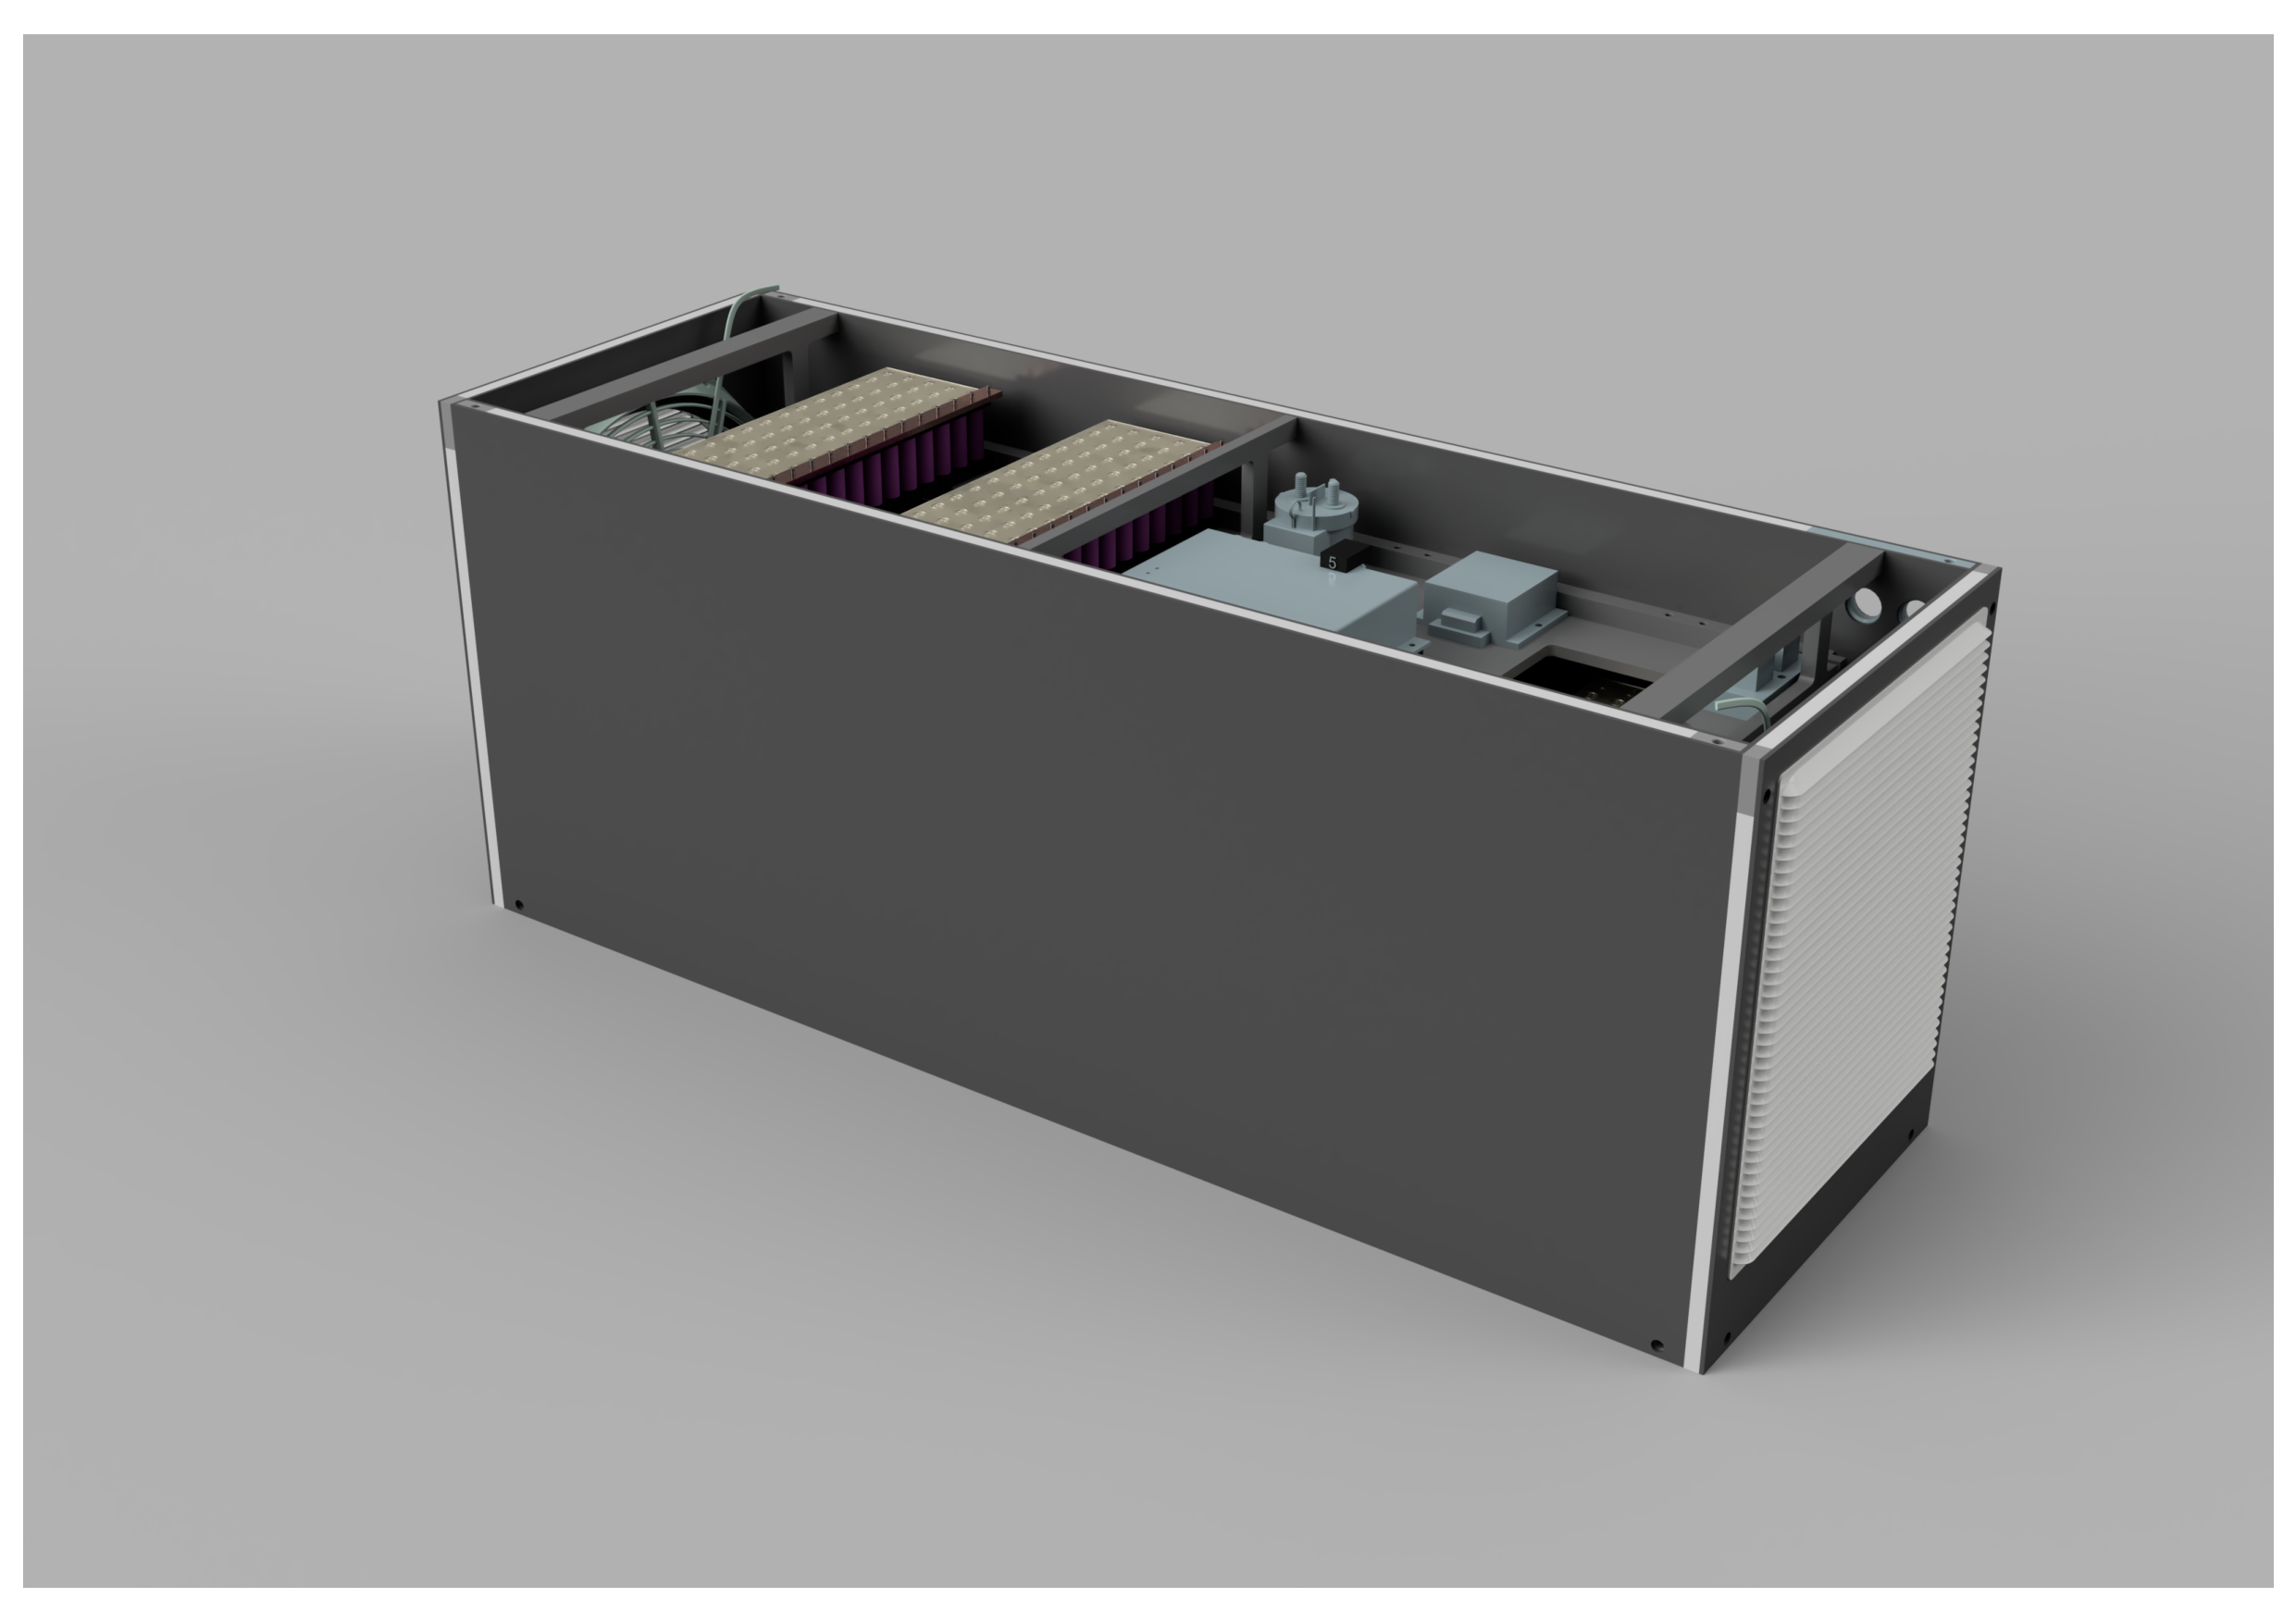
\includepdf[pages=1, fitpaper=true, pagecommand={%
	\thispagestyle{empty}
	\begin{center}
		\captionof{figure}{Fully assembled energy storage module with housing for use in the eMule vehicle.}
		\label{fig:AssemblyHousing}
	\end{center}
}]{circuts/Energiespeichersystem_Assembley_TOP_mit gehause.pdf}
\addtocounter{page}{1}
The final design step was the addition of a functional enclosure as seen in \ref{fig:AssemblyHousing}. The enclosure was modeled as a single shell body with integrated ventilation openings, flanged screw points, and access cutouts for connectors. Its purpose is to protect the cells from mechanical impact, environmental contamination, and unintentional contact.

The enclosure follows the contour of the internal components closely, minimizing unused space while allowing air to circulate between components. To accommodate additive manufacturing constraints, all overhangs were designed with a maximum angle of 45°, and fillets were added at all interior corners to prevent stress concentration. A removable lid was included to enable servicing of the battery.

The following figure illustrates the fully enclosed battery system, ready for 3D printing.

% Assembly mit Gehäuse


\section{Conclusion on the CAD Design Process}

Using Fusion 360 allowed for a highly structured, iterative, and parametric modeling workflow. All geometric relationships between components were carefully maintained, which significantly simplified later adjustments. The use of parametric sketches and pattern tools proved crucial in efficiently laying out large arrays of repetitive features, such as the cell holders.

The final result is a complete digital twin of the battery system, suited for additive manufacturing and integration in the E-Mule platform. While no physical tests or simulations were performed, the model meets the spatial, mechanical, and packaging criteria outlined at the beginning of the project.

